\definecolor{bblue}{HTML}{4F81BD}
\definecolor{rred}{HTML}{C0504D}
\definecolor{ggreen}{HTML}{9BBB59}
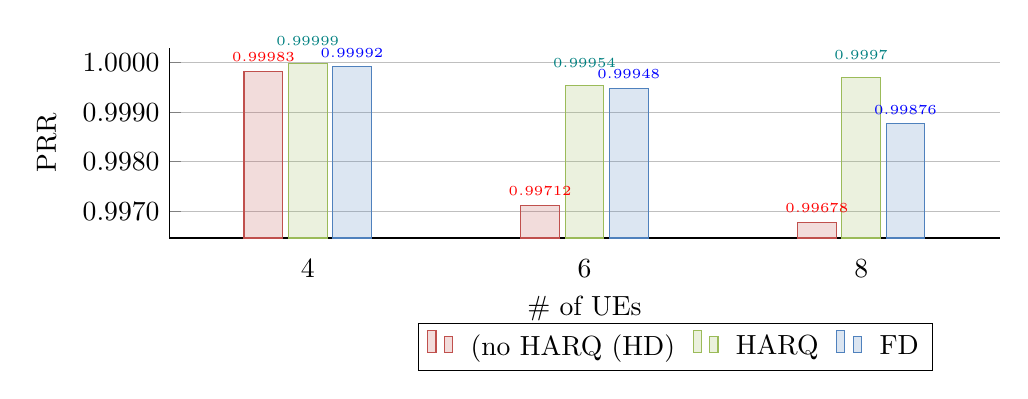
\begin{tikzpicture}
    \begin{axis}[
        width  = \columnwidth,
        height = 4cm,
        major x tick style = transparent,
        ybar,
        %ybar=2*\pgflinewidth,
        bar width=14pt,
        ymajorgrids = true,
        ylabel = {PRR},
        ylabel style={yshift=0.1cm},
        xlabel = {\# of UEs},
        symbolic x coords={4, 6, 8},
        nodes near coords,
        nodes near coords style={fill opacity=1.0,font=\tiny, /pgf/number format/.cd,precision=5},
        %every node near coord/.append style={font=\small},
        xtick = data,
        scaled y ticks = true,
        axis y line*=left,
        axis x line*=bottom,
        enlarge x limits=0.25,
        y tick label style={ /pgf/number format/.cd, fixed, fixed zerofill, precision=4},
        %ymin=0,
        legend columns=-1
        legend cell align=left,
        legend style={
                at={(0.92,-0.7)},
                anchor=south east,
                column sep=1ex
        }
    ]
        \addplot[style={rred,fill=rred, fill opacity=0.2, mark=none, text=red}]
            coordinates {(4, 0.999831) (6, 0.997122) (8, 0.996777)};

        \addplot[style={ggreen,fill=ggreen, fill opacity=0.2, mark=none, text=teal}, nodes near coords=\raisebox{0.1cm}{\pgfmathprintnumber\pgfplotspointmeta}]
             coordinates {(4,0.999986) (6,0.99954) (8,0.9997)};

        \addplot[style={bblue,fill=bblue, fill opacity=0.2, mark=none, text=blue}]
             coordinates {(4,0.999918) (6,0.999483) (8,0.998763)};

        \legend{(no HARQ (HD),HARQ,FD}
    \end{axis}
\end{tikzpicture}